\documentclass{article}

\usepackage{graphicx}
\usepackage{tikz}
\usepackage{tikzsymbols}
\usetikzlibrary{calc,patterns,shapes.geometric}
\pagestyle{empty}
\usepackage[margin=0pt]{geometry}
\geometry{papersize={14in,12in}}

\def\centerarc[#1](#2)(#3:#4:#5){\draw[#1] ($(#2)+({#5*cos(#3)},{#5*sin(#3)})$) arc (#3:#4:#5);}

\begin{document}
	\begin{figure}
		\centering
		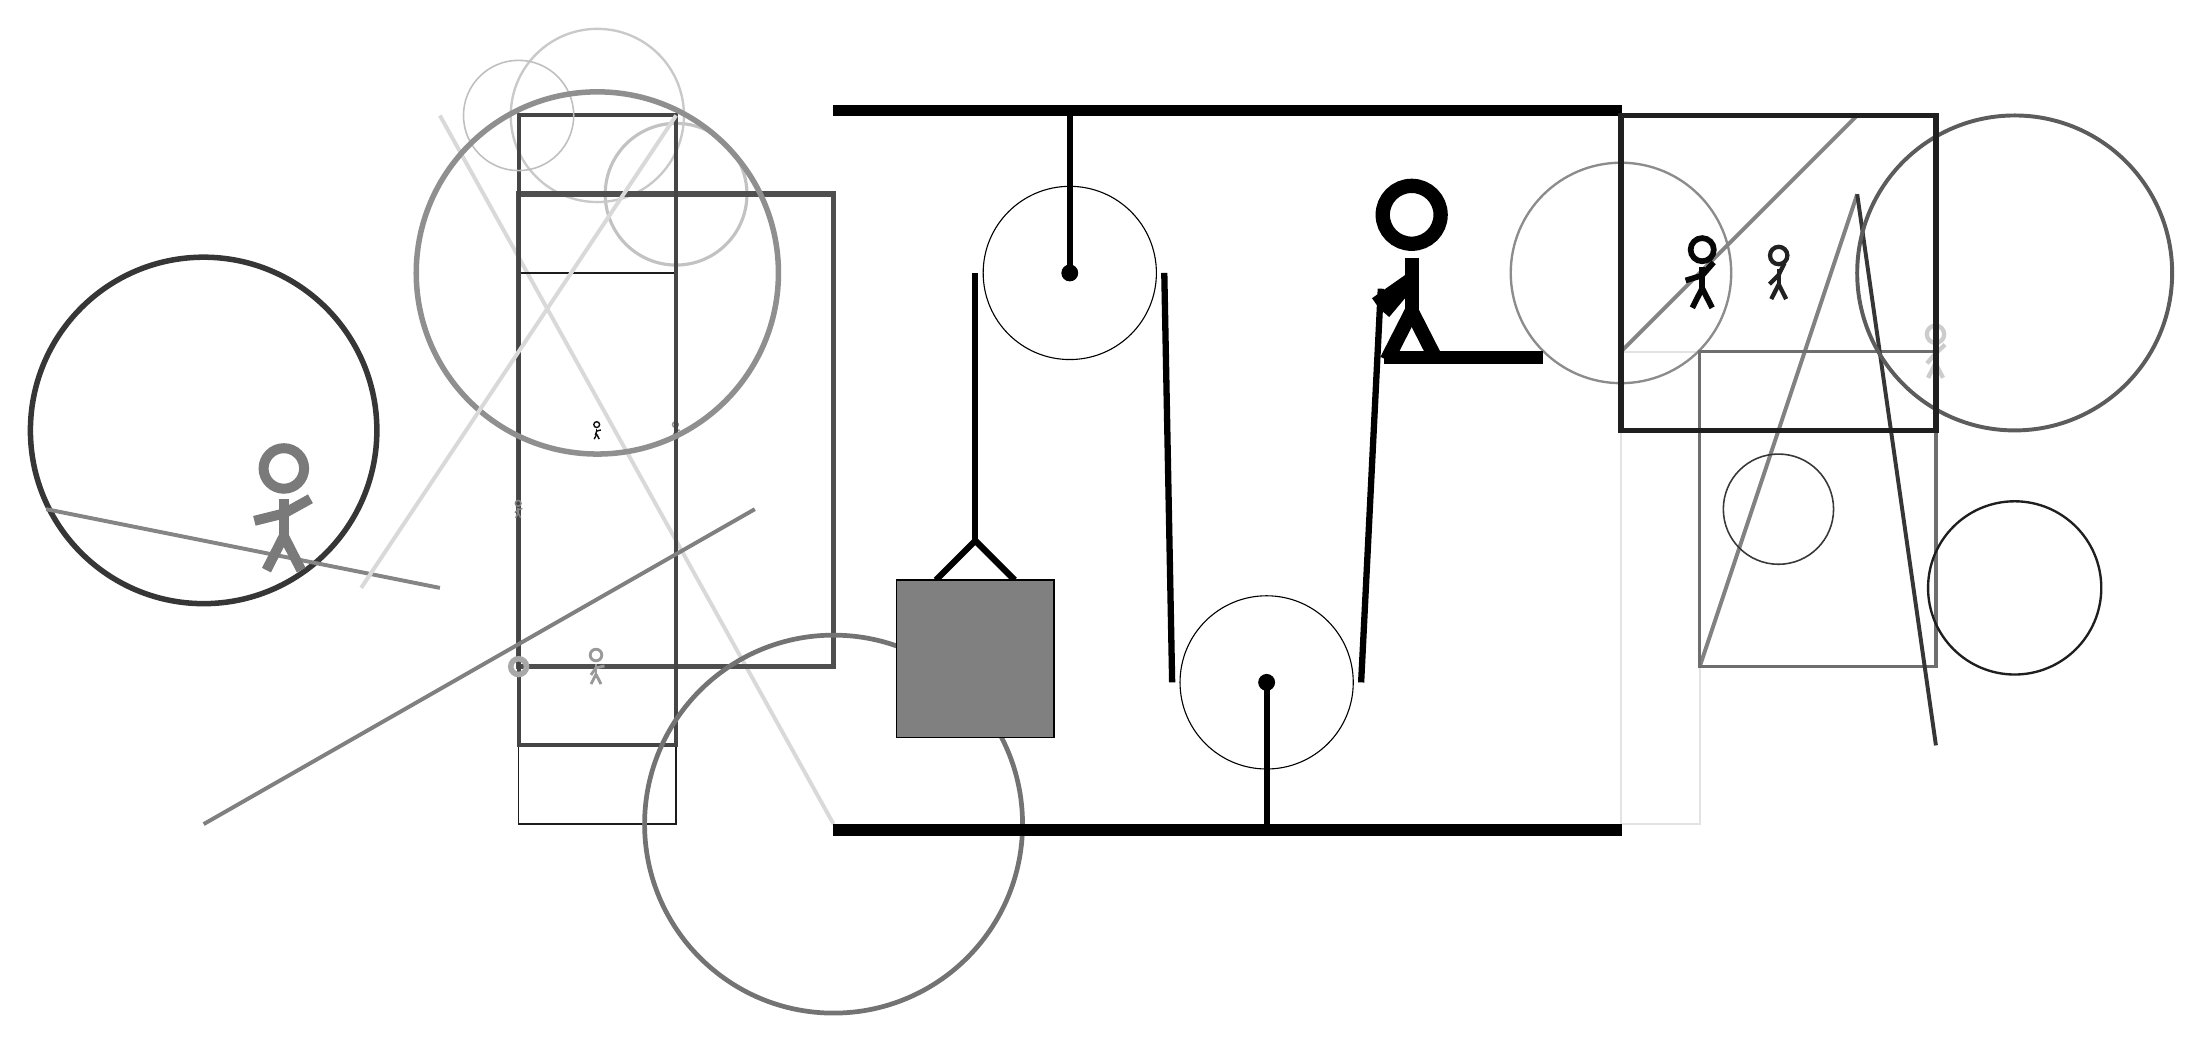
\begin{tikzpicture}
			%%%%% START %%%%%
			
			\draw[fill=black] (-2, 9) rectangle (8, 9.125);
			
			\draw[line width=0.3mm, color=black!11] (8, 6) rectangle (9, 0);
			
			\draw[line width=0.5mm, color=black!56](-4, 3) -- (-4, 5);
			\node[line width=0.6mm, color=black!45] at (-4, 5) {\Strichmaxerl[1][62][15]};
			\draw[line width=0.5mm, color=black!15](-2, 0) -- (-7, 9);
			\node[line width=0.5mm, color=black!87] at (10, 7) {\Strichmaxerl[3][45][64]};
			
			\draw [line width=0.3mm, color=black!45](8, 7) circle (1.4);
			
			\draw[line width=0.5mm, color=black!51](-6, 2) -- (-3, 2);
			\draw [line width=0.4mm, color=black!24](-4, 8) circle (0.9);
			\draw [line width=0.7mm, color=black!79](-10, 5) circle (2.2);
			
			\draw[line width=0.5mm, color=black!49](9, 2) -- (11, 8);
			\draw[line width=0.4mm, color=black!57] (9, 6) rectangle (12, 2);
			\draw[line width=0.5mm, color=black!48](-7, 3) -- (-12, 4);
			\node[line width=0.4mm, color=black!52] at (-9, 4) {\Strichmaxerl[7][14][29]};
			
			\draw [line width=0.3mm, color=black!21](-5, 9) circle (1.1);
			\draw[line width=0.7mm, color=black!69] (-2, 8) rectangle (-6, 2);
			\draw[line width=0.5mm, color=black!48](8, 6) -- (11, 9);
			
			\draw[line width=0.2mm, color=black!89] (-4, 0) rectangle (-6, 7);
			
			\draw [line width=0.2mm, color=black!78](10, 4) circle (0.7);
			\draw[line width=0.5mm, color=black!73] (-4, 9) rectangle (-6, 1);
			
			\draw[line width=0.5mm, color=black!79](12, 1) -- (11, 8);
			\draw [line width=0.6mm, color=black!55](-2, 0) circle (2.4);
			\draw [line width=0.2mm, color=black!25](-6, 9) circle (0.7);
			\node[line width=0.6mm, color=black!40] at (-5, 2) {\Strichmaxerl[2][54][13]};
			\draw[line width=0.5mm, color=black!44](12, 5) -- (12, 8);
			\node[line width=0.7mm, color=black!93] at (-5, 5) {\Strichmaxerl[1][72][14]};
			
			\node[line width=0.5mm, color=black!20] at (12, 6) {\Strichmaxerl[3][49][43]};
			\draw[line width=0.5mm, color=black!50](-3, 4) -- (-10, 0);
			\draw [line width=0.7mm, color=black!44](-5, 7) circle (2.3);
			\draw [line width=0.5mm, color=black!64](13, 7) circle (2.0);
			\node[line width=0.5mm, color=black!97] at (9, 7) {\Strichmaxerl[4][17][49]};
			\draw [line width=0.7mm, color=black!34](-6, 2) circle (0.1);
			\draw[line width=0.7mm, color=black!88] (8, 9) rectangle (12, 5);
			\draw [line width=0.3mm, color=black!88](13, 3) circle (1.1);
			
			\draw[line width=0.5mm, color=black!15](-4, 9) -- (-8, 3);
			
			\node[line width=0.3mm, color=black!48] at (-6, 4) {\Strichmaxerl[1][41][17]};
			
			\draw (3.5, 1.8) circle (1.1);
			\draw[fill=black] (3.5, 1.8) circle (0.1);
			\draw[line width=0.8mm] (3.5, 1.8) -- (3.5, 0);
			
			\draw (1, 7) circle (1.1);
			\draw[fill=black] (1, 7) circle (0.1);
			\draw[line width=0.8mm] (1, 9) -- (1, 7);
			
			\draw[line width=0.8mm](-0.7, 3.1) --  (-0.2, 3.6) -- (0.3, 3.1);
			\draw[fill=black!50] (-1.2, 3.1) rectangle (0.8, 1.1);
			
			\draw[line width=0.8mm](-0.2, 7) -- (-0.2, 3.6);
			\centerarc[line width=0.8mm](1, 7)(180:0:1.2000000000000002)
			\draw[line width=0.8mm](2.2, 7) -- (2.3, 1.8);
			\centerarc[line width=0.8mm](3.5, 1.8)(180:360:1.2000000000000002)
			\draw[line width=0.8mm](4.7, 1.8) -- (4.95, 6.8);
			
			\node at (5.3, 7) {\Strichmaxerl[10][35][-130]};
			\draw[fill=black] (5, 6) rectangle (7, 5.85);
			
			\draw[fill=black] (-2, 0) rectangle (8, -0.15);
			
			%%%%% END %%%%%
		\end{tikzpicture}
	\end{figure}	
\end{document}